\documentclass[11pt, oneside]{article} 
\usepackage{geometry}
\geometry{letterpaper} 
\usepackage{graphicx}
	
\usepackage{amssymb}
\usepackage{amsmath}
\usepackage{parskip}
\usepackage{color}
\usepackage{hyperref}

\graphicspath{{/Users/telliott_admin/Tex/png/}}
% \begin{center} \includegraphics [scale=0.4] {gauss3.png} \end{center}

\title{Fermat and Euler's Theorems}
\date{}

\begin{document}
\maketitle
\Large

\subsection*{theorem}
Fermat's Theorem (often called Fermat's "little" Theorem) says that for any prime number $p$ and any integer $1 < a < n$ 
\[ a^p  \text{ mod } p = a \]
Examples:  $2^3 \text{ mod } 3 = 2$;  $2^5 \text{ mod } 5 = 32  \text{ mod } 5 = 2$;  $3^5 \text{ mod } 5 = 243 \text{ mod } 5 = 3$.

An equivalent statement is
\[ a^{p-1} \text{ mod } p = 1 \]
Consider $p=7$
\begin{verbatim}
1**6       1 mod 7 = 1
2**6 =    64 mod 7 = 1
3**6 =   729 mod 7 = 1
4**6 =  4096 mod 7 = 1
5**6 = 15625 mod 7 = 1
6**6 = 46656 mod 7 = 1
\end{verbatim}
Here is a table from Laws of Cryptography  for $p = 13$, which computes such powers more efficiently (computing mod $7$ at each step).
\begin{center} 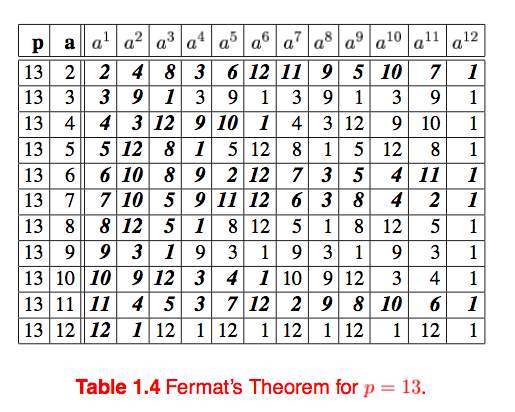
\includegraphics [scale=0.7] {Fermat13.png} \end{center}

\url{www.cs.utsa.edu/~wagner/lawsbookcolor/laws.pdf}

Let's do the calculation for $a = 7, p = 13$:
\begin{verbatim}
7**1  =               7
7**2  = 49 - 3(13) = 10
7**3  = 70 - 5(13) =  5
7**4  = 35 - 2(13) =  9
7**5  = 63 - 4(13) = 11
7**6  = 77 - 5(13) = 12
7**7  = 84 - 6(13) =  6
7**8  = 42 - 3(13) =  3
7**9  = 21 - 1(13) =  8
7**10 = 56 - 4(13) =  4
7**11 = 28 - 2(13) =  2
7**12 = 14 - 1(13) =  1
\end{verbatim}

As the theorem says, we cycle around to $7^{12}$ mod $13 = 1$.  The number $7$ is called a generator because its powers generate all the values in the field $Z_{13}$. 

$2, 6$ and $11$ are also generators for this field.

Other values for $a$ have shorter repeats.  The lengths of these runs are divisors of 12.

As the source says:

\textbf{Because $a$  to a power $x$ mod $p$ always starts repeating after the power reaches $p-1$, one can reduce the power mod $p-1$ and still get the same answer."}

Thus no matter how big the power $x$
\[ a^x \text{ mod } p = a^{x \text{ mod } p-1} \text{ mod } p \]
For example, mod $13$:
\[ a^{29} \text{ mod } 13 = a^{29 \text{ mod } 12} \text{ mod } 13 = a^5  \text{ mod } 13 \]

\subsection*{proof of Fermat's Theorem}

There is a beautiful proof in wikipedia called the "necklace proof".

\subsection*{consequence}

A consequence of this is that the sequence
\[ a^1, a^2, a^3 \dots a^{p-1} \]
repeats, so this sequence
\[ a^{p}, a^{p+1} \dots a^{2p - 1} \]
gives exactly the same values.

\subsection*{Euler}
Euler's totient function $\phi(n)$ is defined like so:
\[ \phi(n) = n \ \prod \ (1 - \frac{1}{p_i}) \]
(with $p_i$ being the prime factors of $n$).  In number theory, $\phi$ is a count of the positive integers up to a given integer $n$ that are relatively prime to $n$ (are not divisors of $n$).

\subsection*{theorem}
Relevant to our study of cryptography, Euler's Theorem says that for an integer $a < p$ (not equal to $1$):
\[ a^{\phi(n)} \text{ mod } n = 1 \]
If $n$ is prime this reduces to 
\[ \phi(n) = n \ \prod (1 - \frac{1}{n}) =  n(1 -  \frac{1}{n}) = n - 1 \]
and then
\[ a^{n-1} \text{ mod } n = 1 \]
giving Fermat's Theorem as a special case of Euler's Theorem.

Here we are more interested in the situation where $n$ has two large prime factors $p$ and $q$ and then:
\[ \phi(n) = pq \ (1 - \frac{1}{p}) (1 - \frac{1}{q}) = (p - 1)(q - 1)  \]
I will write $\phi$ for $\phi(n)$ from now on.

Furthermore, we have that encryption followed by decryption is $m^{ed} \text{ mod } n = m$.  We would like to show that this follows as a consequence of our definitions.  

Recall that we set $d$ to be the multiplicative inverse of $e$ mod $\phi$. 

Write out what's given:
\[ \phi = (p - 1)(q - 1) \]
\[ m^{\phi} \text{ mod } n = 1 \]
\[ ed  \text{ mod } \phi = 1 \]
And our encryption/decryption is $(m^{e})^{d}$ mod $n$  or:
\[ m^{ed} \text{ mod } n \]

My source says:  "similar to Fermat's Theorem, arithmetic in the exponent is taken mod $\phi$."  

So the idea is that since  
\[ m^{\phi} \text{ mod } n = 1 \]
if we are computing any \emph{other} power of $m$, say $ed$, we need only compute to the $ed$ mod $\phi$ power, because beyond that, the sequence just repeats.

So, (assuming $m$ has no common divisors with $n$):
\[ m^{ed} \text{ mod } n = m^{ed \text{ mod } \phi} \ \text{ mod } n \]
But of course $ed \text{ mod } \phi = 1$ so this is just $m$.

Furthermore, $m^{ed} = m^{de}$, hence the ability to encrypt first with the private key and then decrypt with the public one.

\end{document}  